
Given the results of
direct simulation it is
possible to examine
the approximations
used to arrive at
the Lindblad equation.

\subsection{Single State Tunnelling Rate}\label{sec:Lindblad corrected tunneling}
When simulating the
degenerate hydrogen tunneling in
\cref{sec:degenerate tunnelling simulaton}
we found that the tunneling rate
grew proportional to \(4R_0N(1-N)\).
This corresponds exactly to the
form of the integrand of
\cref{eqn:gamma integral form},
which was proportional to
\(N_1(1 - N_3)\) where
\(E_{k3} = E_{k1} + \omega{}\),
and \(\omega{}\) is equal to
the difference in hydrogen energies
\begin{equation}
    \Gamma_{i,j, k,l}(\omega)  =\begin{aligned}[t]
        4 \int &
        \frac{d^3\vec{k}_1}{{(2\pi)}^3}
        \frac{d^3\vec{k}_3}{{(2\pi)}^3}
        V_{i,j} V_{k,l}
        N_1 (1 - N_3)
        \frac{m\delta({k_3 \pm \sqrt{k_1^2 + 2m\omega}})}{\sqrt{k_1^2 - 2m\omega}}
    \end{aligned}
\end{equation}
This suggests
that the process
is dominated
by single electron
transitions, an assumption
that was made in \cref{eqn:second order eqn of motion}
when expanding the equation
of motion to second order.

If we were to look at the
tunneling for \(\omega \neq 0\)
we find that the correct
way to modify the tunneling
rate in the simulation should
be to set
\(R(N\rightarrow{}N') = 2R_0N(1-N')\)
corresponding to \cref{eqn:target correction rate}
in
\cref{sec:corrected transition rate}.


\subsection{Final State Correction}
In \cref{sec:simulation results} we argued
that the electron state immediately
after a transition
should not effect the
dynamics of the system,
however in the Lindblad
analysis it should be possible to
properly take into account
the change in electron
distributions through
the introducing a coupling between
the electron and hydrogen density
matrices.
Although this a difficult
problem in general
if we were
to introduce a coupling
\begin{equation}
    \hat{\rho}_t = \sum_{m,n} \hat{\rho}_{m,n} \otimes {(\hat{\rho}_E)}_{m,n} \
\end{equation}
we can follow the same procedure as in
\cref{sec:the redfield assumption}
to arrive at a modified redfield equation
\begin{equation}
    \bra{m}\dot{\hat{\rho}}(t)\ket{n} = \begin{aligned}[t]
        \sum_{i,j,k, l} &
        \exp{(-i(\omega_{i,j}-\omega_{k,l})t)}
        \Gamma^{m,n}_{i,j;k, l}(\omega_{k,l})
        [S_{k, l}{\hat{\rho}(t)}_{m,n},
        S^\dagger_{i,j}]  \\
        +               &
        \exp{(i(\omega_{i,j}-\omega_{k,l}))}
        {\Gamma^*}^{m,n}_{k, l; i,j}(\omega_{i,j})
        [S_{k, l},
                {\hat{\rho}(t)}_{m,n} S^\dagger_{i,j}]
    \end{aligned}
\end{equation}
where
\begin{equation}
    \Gamma^{m,n}_{i,j, k,l}(\omega) =
    \int_0^\infty{}{
    ds \exp{(i\omega{}s)}
    Tr_{E}[E^\dagger_{i,j}(t)E_{k,l}(t-s)
    {(\hat{\rho}_E)}_{m,n}]
    }
\end{equation}
The problem is then how best to express
both the statistical and quantum uncertainty
in the form of a density matrix.

\subsection{Rotating Wave Approximation}\label{sec:rotating wave approximation}
If we relax the rotating wave approximation
made in \cref{sec:Lindblad equation}
we arrive at the full Redfield equation
(\cref{sec:redfield equation full solution}).
\begin{align}
    \bra{m}\dot{\hat{\rho{}}}(t) \ket{n} & = \begin{aligned}[t]
        \sum_{i,j} &
        \exp{(-i\Delta{}E_{n,j;m,i} t)}
        \Gamma_{n,j;m, i}(\omega_{m,i})
        \rho_{i,j}   \\
                   &
        -\exp{(-i\Delta{}E_{i,m;i,j} t)}
        \Gamma_{i,m;i, j}(\omega_{i,j})
        \rho_{j, n}  \\
                   &
        +\exp{(i\Delta{}E_{n,j;m,i} t)}
        \Gamma_{n,j; m, i}(\omega_{n,j})
        \rho_{i, j}  \\
                   &
        -\exp{(i\Delta{}E_{i,j;i,n} t)}
        \Gamma_{i,j; i, n}(\omega_{i,j})
        \rho_{m, j}
    \end{aligned}
\end{align}
This equation produces extra oscillations
on top of the Lindblad result, with
a characteristic timescales of
\(\frac{2\pi}{\omega_{1,0}} = 2.13\times{}10^{-13}s\). Plotting
the full solution (\cref{fig:redfield full solution})
we see exactly the same behaviour as that
predicted by the Lindblad result.
\begin{figure}[htbp]
    \centering
    \begin{subfigure}{0.45\linewidth}
        \centering
        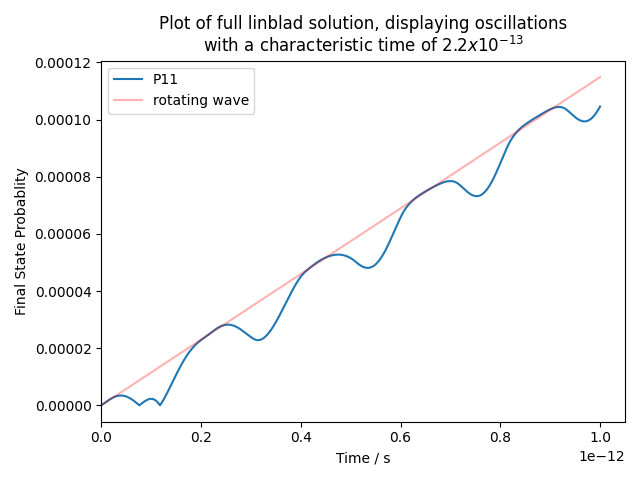
\includegraphics[width =0.9 \linewidth]{Figures/Redfield/Plot of redfield solution short time.png}
        \caption{Complete solution for small times
        }\label{fig:redfield full solution short timescales}
    \end{subfigure}
    \hfill
    \begin{subfigure}{0.45\linewidth}
        \centering
        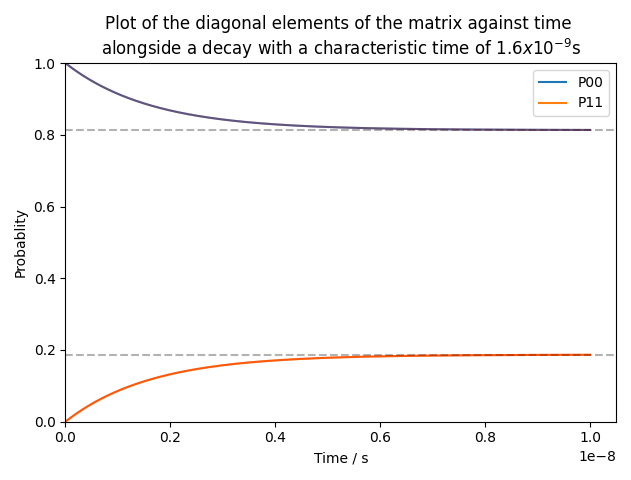
\includegraphics[width = 0.9\linewidth]{Figures/Redfield/Plot of redfield solution long time.png}
        \caption{Complete solution for long times
        }\label{fig:redfield full solution long timescales}
    \end{subfigure}
    \begin{subfigure}{0.45\linewidth}
        \centering
        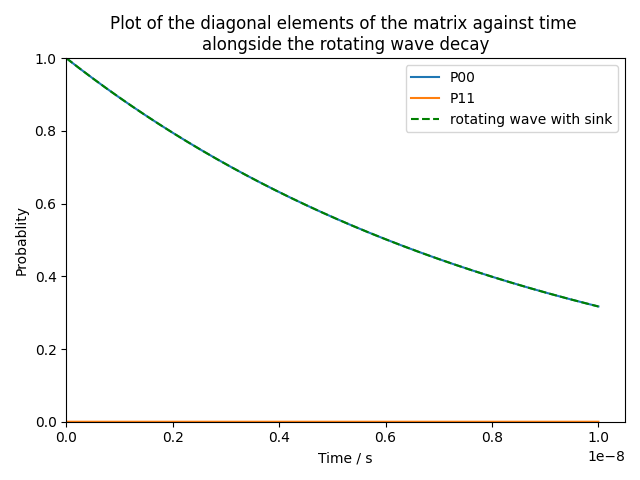
\includegraphics[width = 0.9\linewidth]{Figures/Redfield/Plot of redfield solution long time sink.png}
        \caption{Complete solution with sink
        }\label{fig:redfield full solution with sink}
    \end{subfigure}
    \caption{Plot of the full solution of the Redfield
    equation. On short timescales
    (\cref{fig:redfield full solution short timescales})
    the solution is seen to
    oscillate with a characteristic
    frequency of \(2.1\times{}10^{-13}\)s however
    at long timescales
    (\cref{fig:redfield full solution long timescales})
    the solution decays at the same rate as the
    Lindblad equation. The solution is
    also well behaved with the inclusion of
    a sink at the HCP site
    (\cref{fig:redfield full solution with sink}).
    }\label{fig:redfield full solution}
\end{figure}
In theory we should also be able
to solve the redfield equation
for multiple hydrogen sites, however
the additional computational complexity
rules this out. It is possible to
approximate the behaviour
seen in the many site model
by placing a sink at
the HCP site
(\cref{fig:redfield full solution with sink}).
In this case
we again see good
agreement with the
Lindblad equation.


\subsection{Separable Density matrix}
In the analysis of the Lindblad
equation we also assumed that is was possible
to factorise the density
matrix
\begin{equation}
    \hat{\rho}_t(t) = \hat{\rho}(t) \otimes \hat{\rho}_E(0)
\end{equation}
It is clear from the
initial and final
state energy distribution that
in the limit of a large
number of states the
diagonal elements are completely
uncorrelated with the
hydrogen occupation.
In the real simulation
the electron density
matrix is not diagonal,
however if we average
over a small period of time
the average is seen to
fall to zero
(\cref{fig:density matrix analysis}).
\begin{figure}[htbp]
    \centering
    \begin{subfigure}{0.45\linewidth}
        \centering
        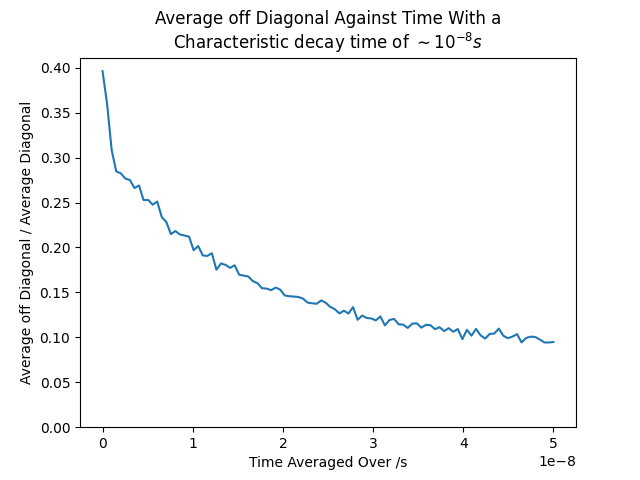
\includegraphics[width =0.9 \linewidth]{Figures/Discussion/Off Diagonal Average Matrix Element Decay.png}
        \caption{Average Off-Diagonal Decay
        }\label{sub@fig:off diagonal matrix decay}
    \end{subfigure}
    \hfill
    \begin{subfigure}{0.45\linewidth}
        \centering
        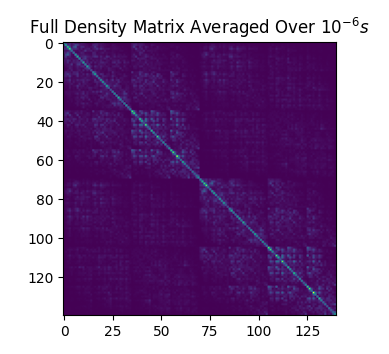
\includegraphics[width = 0.9\linewidth]{Figures/Discussion/Full average matrix 10-6s.png} %ChkTeX 8
        \caption{Averaged Density Matrix
        }\label{sub@fig:averaged density matrix}
    \end{subfigure}
    \caption{
    Plot of the average
    electron density matrix
    for a system of 5 electrons
    and 10 states
    corresponding to a tunneling time
    of \(\sim 2\times{}10^{-4}s\).
    The average off diagonal
    elements can be seen to
    fall in around
    \(\sim 2\times{}10^{-8}s\).
    }\label{fig:density matrix analysis}
\end{figure}
The approximation
therefore holds for the
same reason we are able
to ignore the off-diagonal
terms in the hydrogen density
matrix
(\cref{sec:rotating wave approximation}).
Since
the off diagonal terms
oscillate at much shorter
timescales they have
no effect on the dynamics
of the system.

\subsection{Q Dependance}
For this report we use a
q-independent model of the
electron hydrogen interaction.
If we instead include the full form
of the interaction potential
into \cref{eqn:gamma integral form}
we find a
Lindblad rate constant that
is \(0.418 \times{}\) that
previously calculated.

We also expect a
contribution from the
\(\vec{q}\) dependance of the hydrogen overlap
fourier transform, however
to
include this we would need to
convert the discrete
DFT calculations into a continuous
function of \(\vec{q}\).
It is also possible that
the rapid oscillations
seen in the fourier transform
are simply artifacts of the
discrete DFT analysis.

For the  simulation
it will always
be necessary to assume a
\(\vec{q}\)-independent
matrix element in general,
as it is not possible
to include enough
states to properly
sample all possible initial
and final
states in 3D.
The corrections made in
the Lindblad analysis could
be applied to the simulation,
producing an effective matrix
element depending only
on the energy difference between
two states.


\subsection{Realistic Treatment of Electrons}
In the development
of the electron-hydrogen
model we also assumed
an ideal electron gas,
with a fermi energy
of \(1.91\times{}10^{-18}J\).
The real fermi energy
of nickel actually slightly lower,
at only \(1.24\times{} 10^{-18}J\),
possibly since the two
valence electrons are not
fully delocalised.
The fermi surface of nickel
is also not entirely
spherical~\cite{FermiSufaceNickel},
indeed it is different
for each spin.
This is the cause of
ferromagnetic properties
within the metal~\cite{PhysRev.49.537}.

This behaviour could
be included in the
Lindblad analysis through
a modification of \cref{eqn:gamma integral form},
however it is not possible
to incorporate any
non-spherical behaviour
into the simulation
without the introduction of
an effective constant.
The complex nature of
the nickel band-structure
means that this
could favour low or
high \(\vec{q}\) scattering,
which would lead to either an increase
or decrease in the
overall rate.
The hope
is that the surface
is sufficiently
`smoothed out' by
excitations at high
temperature such that
this is only a small
correction.